\documentclass{article}
\usepackage[utf8]{inputenc}
\usepackage{listings}
\usepackage{xcolor}
\usepackage{amsmath, amssymb}
\usepackage{tabularx}
\usepackage{graphicx}

\title{Git Guide}
\author{Alexandru Andrei Colacel}
\date{\today}

\begin{document}

\maketitle


\section*{Git}
I file in Git possono essere in tre stati principali: modified (modificati), staged (in stage) e committed (committati).
\begin{itemize}
    \item \textbf{Modificato} significa che il file è stato modificato, ma non è ancora stato committato nel database. 
    \item In \textbf{stage} significa che hai contrassegnato un file, modificato nella versione corrente, perché venga inserito nello snapshot alla prossima commit. 
    \item \textbf{Committato} significa che il file è registrato al sicuro nel database locale.
\end{itemize} 

\subsection*{Aggiungere nome ed e-mail}
\begin{itemize}
    \item Aprire la linea di comando
    \item Settare il proprio user name digitando:
    \begin{verbatim}    
        git config --global user.name "FIRST_NAME LAST_NAME"
    \end{verbatim}
    \item Settare la propria email: 
    \begin{verbatim}
        git config --global user.email "MY_NAME@example.com"
    \end{verbatim}    
\end{itemize}

\subsection*{Controllare nome ed e-mail}
\begin{itemize}
    \item Aprire la linea di comando
    \item Controllare il proprio user name digitando:
    \begin{verbatim}    
        git config --global user.name
    \end{verbatim}
    \item Controllare la propria email: 
    \begin{verbatim}
        git config --global user.email
    \end{verbatim}    
\end{itemize}


\subsection*{Comandi}
\subsubsection*{Inizializiamo una repository di una directory esistente}
Se abbiamo una directory già esistente allora possiamo eseguire
\begin{verbatim}
    $ git init
\end{verbatim}
Questo crea una nuova subdirectory chiamata \texttt{.git} che contiente tutti gli eelmenti necessari ai file della repository. Ma a questo punto ancora nessun cambiamento del nostro progetto non è tracciato.
Se vogliamo iniziare a controllare le versioni dei file esistenti dovremmo fare un \texttt{git add} specificando il file che vogliamo aggiungere.
\begin{verbatim}
    $ git add *.c
    $ git add LICENSE
    $ git commit -m 'initial project version'
\end{verbatim}



\subsubsection*{Committiamo i cambiamenti}
Dobbiamo precisare che ai cambiamenti verranno aggiunti solo i file che abbiamo aggiunto con \texttt{git add}. Ora eseguiamo: 
\begin{verbatim}
    $ git commit
\end{verbatim}

Ora per modificare il file di configurazione di git dobbiamo eseguire:

\begin{verbatim}
    $ code ~/.gitconfig
\end{verbatim}


\subsection*{Controllare lo status dei nostri files}
Il comando principale da usare per determinare quali file sono stati aggiunti e per determinare lo stato nel quale si trovano bisogna usare il comando:
\begin{verbatim}
    $ git status
\end{verbatim}

Il comando \texttt{git log} visualizza tutti i commit nella cronologia di una repository. Eseguendo quindi:
\begin{verbatim}
    $ git log
\end{verbatim}
Visualizzeremo:
\begin{itemize}
    \item Secure Hash Algorithm (SHA)
    \item autore
    \item data
    \item messaggio di commit
\end{itemize}


\subsection*{Come ripristinare un percorso}
Se ci siamo resi conto che un certo \texttt{commit} non era necessario allora dobbiamo prendere la lista degli hash con il comando:
\begin{verbatim}
    $ git log --online
        436ad25 (HEAD -> master) update
        0d014f0 Aggiunto nuovi file
\end{verbatim}
e poi dobbiamo eseguire:
\begin{verbatim}
    $ git checkout 0d014f0
\end{verbatim}

\subsection*{Git Revert e Git Reset (soft, mixed, hard)}
Permette di tornare indietro nel tempo. Il primo comando è:
\begin{verbatim}
    $ git reset --mixed 0d014f0
        o
    $ git reset --soft 0d014f0
        o
    $ git reset --hard 0d014f0
     
\end{verbatim}

\subsubsection*{Ignoriamo dei Files o Directory con Git}
Bisogna creare un file \texttt{.gitignore} e inserire il path da ignorare.

\section*{Come gestire una repository su GitHub da CLI}
\subsection*{Push}
Creare una nuova repository:
\begin{verbatim}
    $ git init
    $ git add FILE.extension
    $ git commit -m "first commit"
    $ git remote add origin https://gitub.com/NOME_SU_GITHUB/NOME_PROGETTO.git
    $ git push -u origin master
\end{verbatim}

Aggiungere ad una repository esistente:
\begin{verbatim}
    $ git remote add origin https://gitub.com/NOME_SU_GITHUB/NOME_PROGETTO.git
    $ git push -u origin master
\end{verbatim}

\subsection*{Pull}
Il comando per scaricare gli aggiornamenti ai file sono:
\begin{verbatim}
    $ git pull origin master
\end{verbatim}

\section*{Cos'è un Branch}
\begin{figure}[hbt]
    \begin{center}
        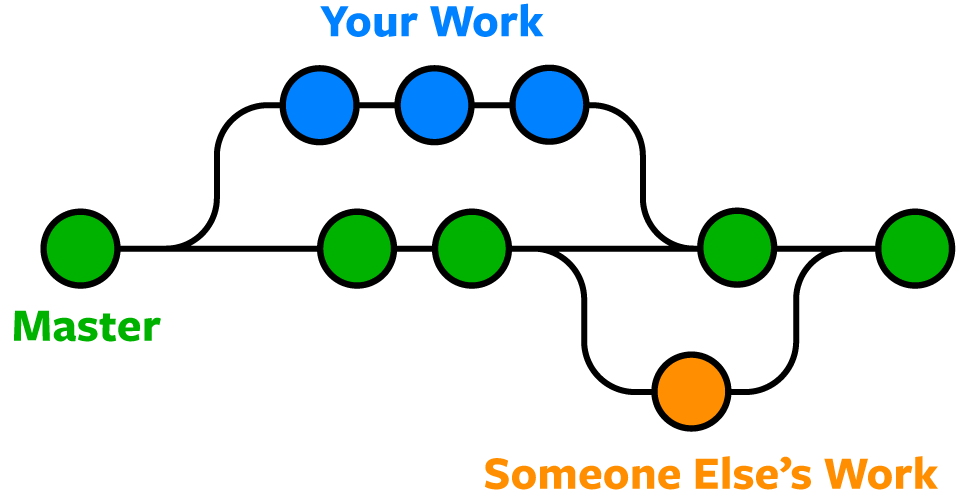
\includegraphics[width=0.8\textwidth,keepaspectratio]{{img/git-branches}}
    \end{center}
    \end{figure}

Creare un nuovo branch aiuta a organizzare il lavoro e permettere il lavoro di diversi utenti. Il comando per la creazione di un nuovo branch:
\begin{verbatim}
    $ git branch NOME-BRANCH
\end{verbatim}

Una volta effettuati tutti i cambiamenti dobbiamo fare il \texttt{commit} su questo branch e poi il \texttt{push}.

Eliminare da GitHub il branch bisogna eseguire:
\begin{verbatim}
    $ git push origin --delete NOME_BRANCH
\end{verbatim}
Ma per elimminarlo anche in locale bisogna prima fare lo switch al branch \texttt{master} con \texttt{git checkout master} e poi eliminare con:
\begin{verbatim}
    $ git branch -D NOME_BRANCH_DA_ELIMINARE
\end{verbatim}

\subsection*{Git merge}
Una volta soddisfatti dei nostri cambiamenti possiamo fare il \texttt{merge}:
\begin{verbatim}
    $ git merge NOME_BRANCH_CREATO
\end{verbatim}


\end{document}
